\documentclass[a4paper,12pt]{article}
\addtolength{\oddsidemargin}{-1.cm}
\addtolength{\textwidth}{2cm}
\addtolength{\topmargin}{-2cm}
\addtolength{\textheight}{3.5cm}
\newcommand{\HRule}{\rule{\linewidth}{0.5mm}}
\makeindex

\usepackage{longtable}
\usepackage[pdftex]{graphicx}
\usepackage{makeidx}
\usepackage{hyperref}
\usepackage{verbatim}
\hypersetup{
    colorlinks=true,
    linkcolor=blue,
    filecolor=magenta,      
    urlcolor=cyan,
}


% define the title
\author{IMAPKD}
\title{ Project Tender}
\begin{document}
\setlength{\parskip}{6pt}

% generates the title
\begin{titlepage}

\begin{center}
% Upper part of the page       

\includegraphics[width=1\textwidth]{./University_of_Pretoria_Logo.PNG}\\[0.4cm]  
\textsc{\LARGE COS 301}\\[0.9cm]
\textsc{\LARGE Department Of Computer Science}\\[0.3cm]

%Title

\HRule \\[0.4cm]
{ \huge \bfseries Application Design and Functional Requirements}\\[0.1cm]
\HRule \\[0.4cm]  

% Group Members 

\begin{minipage}{0.4\textwidth}
\begin{flushleft} \large

\emph{\Large Group Members:}\\[0.4cm]    
\emph{}\\
{\Large Diana {Obo}} \\
\emph{}\\
\emph{}\\
{\Large Priscilla {Madigoe}}\\
\emph{}\\
\emph{}\\
{\Large Kudzai {Muranga}} \\
\emph{}\\
\emph{}\\
{\Large Sandile {Khumalo}}\\
\emph{}\\
\emph{}\\

\end{flushleft}
\end{minipage}
\begin{minipage}{0.4\textwidth}
\begin{flushright} \large

\emph{ \Large Student numbers:} \\[0.4cm]  
\emph{}\\
{\Large u13134885}\\
\emph{}\\
\emph{}\\
{\Large u13049128}\\
\emph{}\\
\emph{}\\
{\Large u13278012}\\
\emph{}\\
\emph{}\\
{\Large u12031748}\\
\emph{}\\
\emph{}\\

\end{flushright}
\end{minipage}

% bottom section of title page

{\large \today}
\end{center}
\end{titlepage}
\renewcommand{\thesection}{\arabic{section}}

\newpage
\begin{center}
\textsc{\Large IMPAKD link}\\[0.5cm]
For further references see \href{https://github.com/u13278012/IMPAKD/}{gitHub}.
\today
\end{center}
\newpage
\tableofcontents{}

\newpage
%Kudzai's Section (Vision and Background) - Start 
\section{Vision}
The Property Investor Optimizer project is objective is to evaluate whether a certain rental property is worth buying. It does this by calculating the Return of Investment (ROI) of a property, which can be compared with another property's ROI, to assist a user to optimize their investment strategy according to their portfolio.\\\\
The project will assist the user by helping to answer the following questions:\begin{itemize}
	\item Given a certain bond (interest rate, deposit as a percentage of property value), rental (occupancy rate, agent commission, rental amount) and environmental conditions (Interest rate, inflation) what is the ROI?
	\item When is it better to pay a higher or lower deposit for a bond?
	\item Between two rental scenarios which provides the greater ROI?
	\item Is it better to try and pay off the bond as fast as possible by paying in extra capital?
	\item How does purchasing another property influence a user's ROI and at which point would this be a good idea?
	\item At which point does it make sense to buy another property?
	\item How much tax will the user have to pay?

\end{itemize}
\newpage
\section{Background}
The project was given to us by our client, CSIR, so that we can research how the ROI of different configurations of rental properties can answer the questions listed in the Vision section of this document. Answers to these questions can be used to help users of the system choose to buy the best property that fits their portfolio and requirements with the ease of not having to manually evaluate the property themselves. The project can also be used for property-related research.

%Kudzai's Section (Vision and Background) - Stop

\newpage
\section{Functional Requirements and Application Design}

% Priscilla's Section (Use Case Prioritization) - Start
\subsection{Use case prioritization}
 \underline{\textbf{Critical:}}
	\begin{itemize}
		\item \underline{Property}
			\begin{enumerate}
				\item updateProperty
				\item addProperty
				\item deleteProperty
				\item viewProperty
				\item compareTwoProperties
			\end{enumerate}
		\item \underline{Accounting}
			\begin{enumerate}
				\item calculateNPV
				\item calculateROI
			\end{enumerate}
	\end{itemize}

\underline{\textbf{Important:}}
	\begin{itemize}
		\item \underline{Profile}
			\begin{enumerate}
				\item login
				\item logout
				\item register
				\item viewProfile
				\item updateProfile
			\end {enumerate}

	\end{itemize}

\underline{\textbf{Nice-to-have:}}
	\begin{itemize}
		\item \underline{Report}
			\begin{enumerate}
				\item generateReport
				\item producePDF
				\item viewReport
			\end{enumerate}
	\end{itemize}
% Priscilla's Section (Use Case Prioritization) - End

% Diana Section - START
\subsection{Use case/Services contracts}
\subsubsection{Profile}
	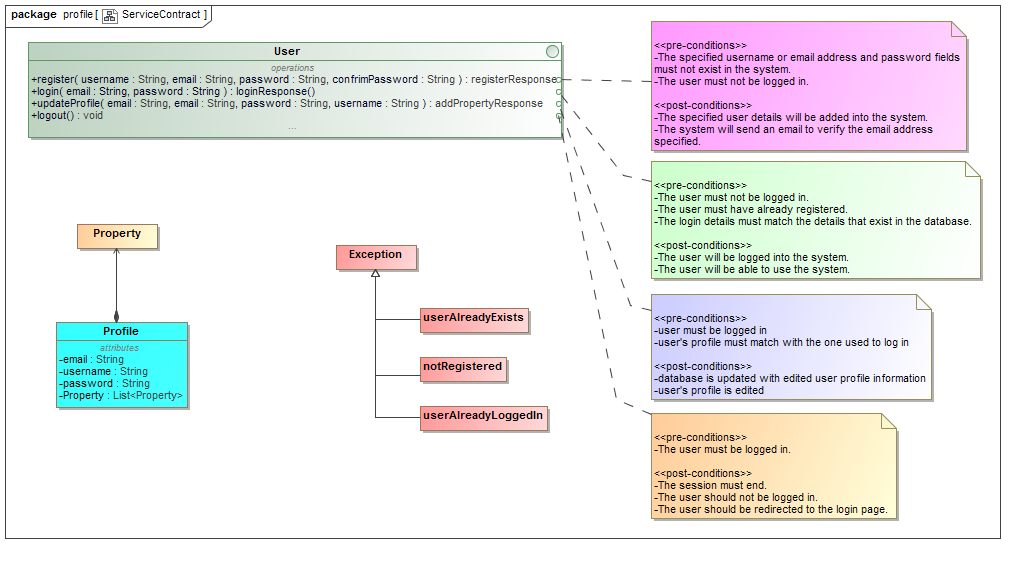
\includegraphics[width=1\textwidth]{./Images/newDiagrams/serviceContract/ServiceContract.png}
% Diana Section - END

% Kudzai's Section - START
\subsubsection{Property}
\textbf{\large{updateProperty}} 

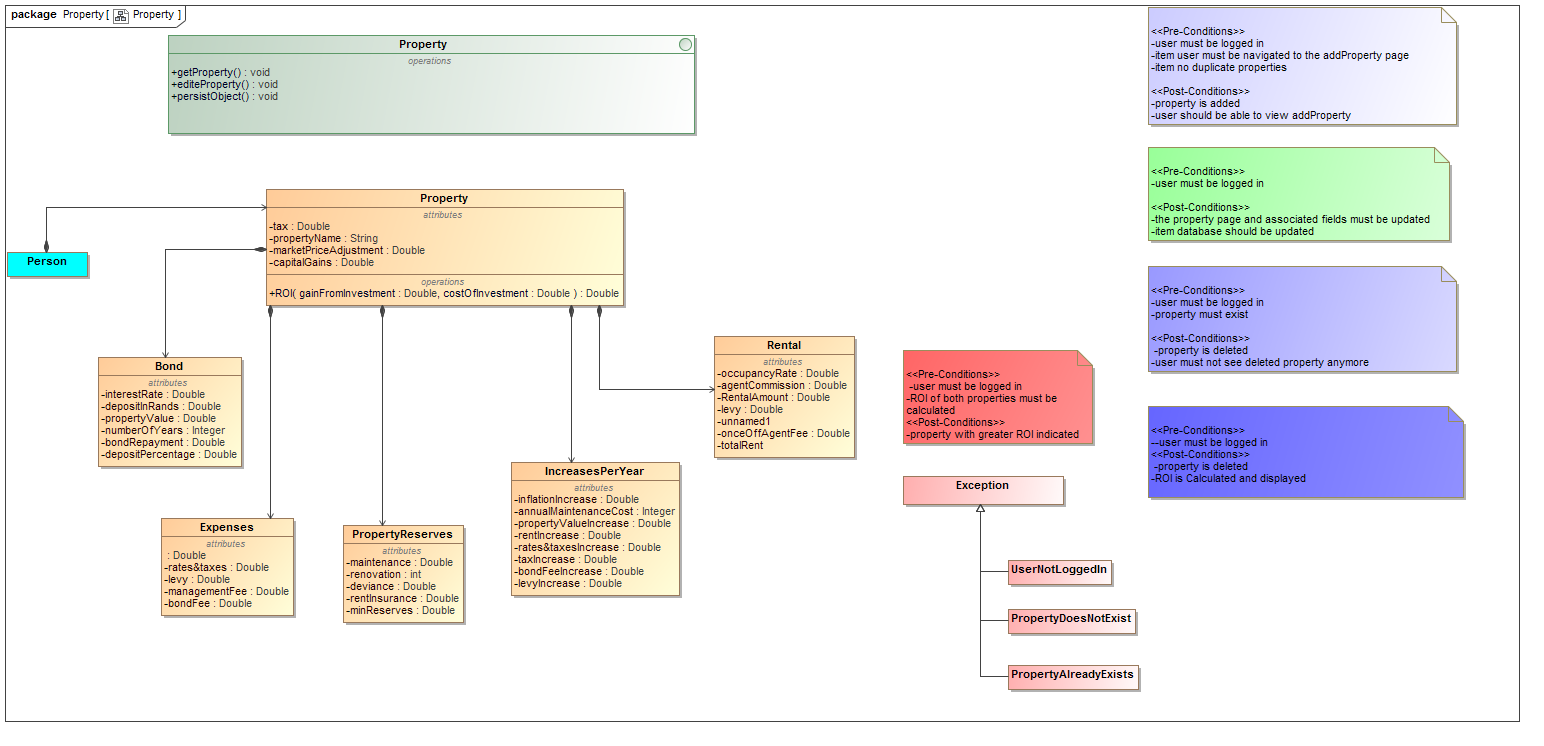
\includegraphics[width=1\textwidth]{./Images/newDiagrams/serviceContract/Property.png} 
% Kudzai's Section - START

%Priscilla's Section (Service Contracts) - Start
\subsubsection{Accounting}
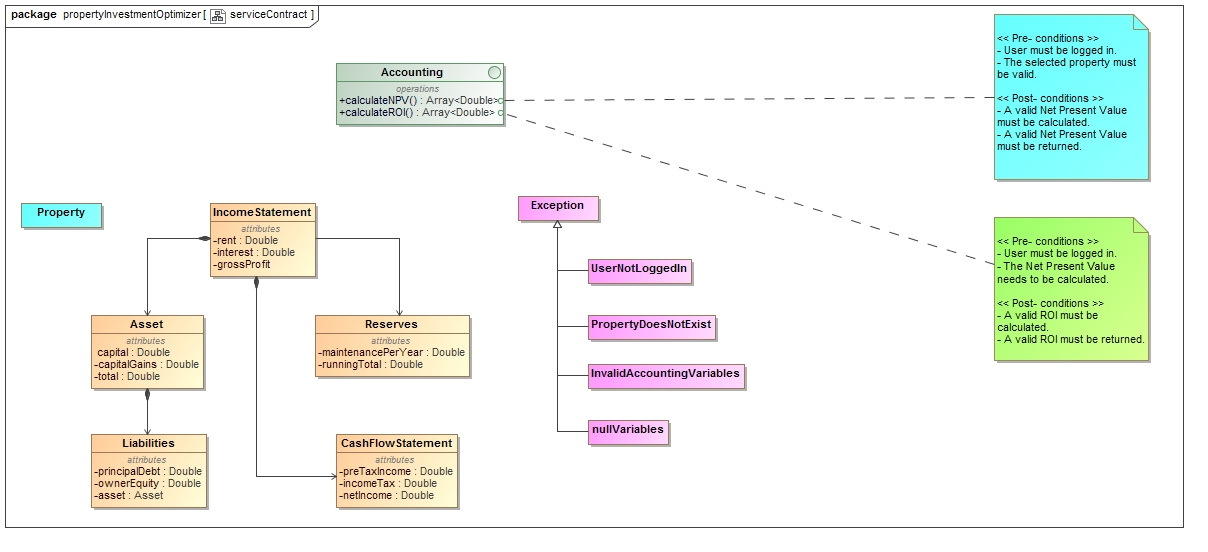
\includegraphics[width=1\textwidth]{./Images/newDiagrams/serviceContract/Priscilla/serviceContract.jpg}
%Priscilla's Section (Service Contracts) - End

%Sandile's Section - START
\subsubsection{Report}
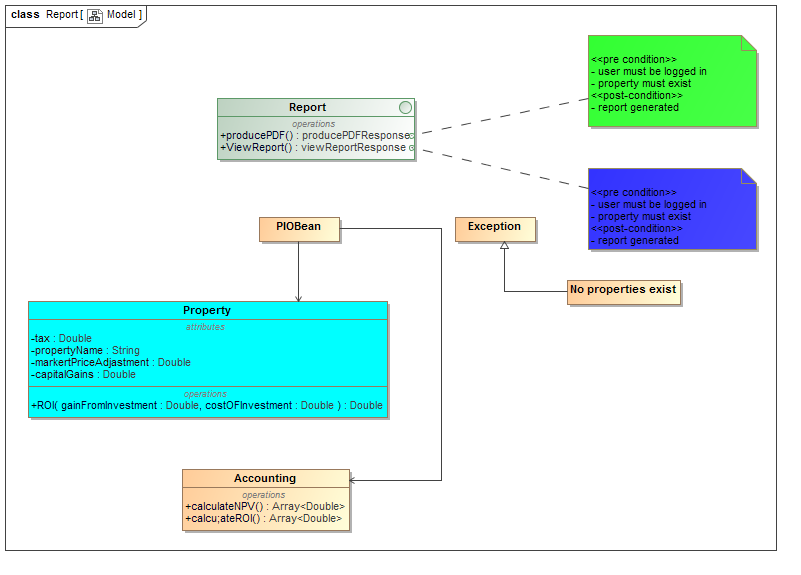
\includegraphics[width=1\textwidth]{./Images/newDiagrams/serviceContract/ReportServiceContract.png}
%Sandile's Section - END

\subsection{Required functionality}
%Diana's Section - Start
\subsubsection{Login}
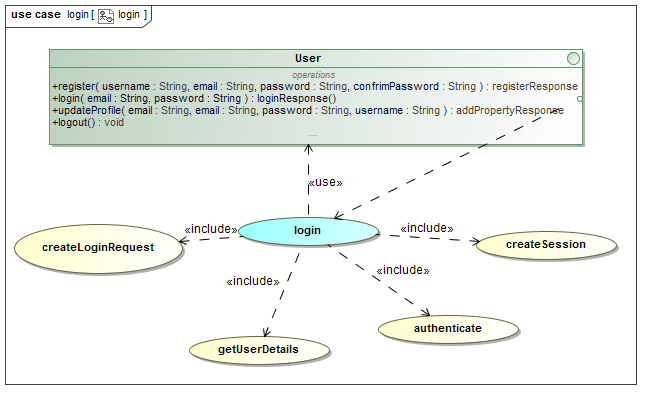
\includegraphics[width=1\textwidth]{./Images/newDiagrams/requiredFunctionality/Diana/login.png}
\subsubsection{Logout}
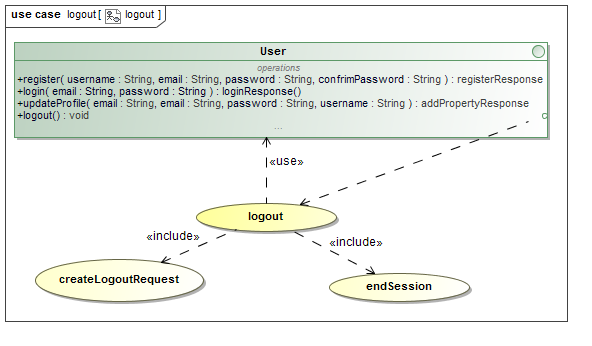
\includegraphics[width=1\textwidth]{./Images/newDiagrams/requiredFunctionality/Diana/logout.png}
\subsubsection{Register}
\includegraphics[width=1\textwidth]{./Images/newDiagrams/requiredFunctionality/Diana/register.png}
\subsubsection{updateProfile}
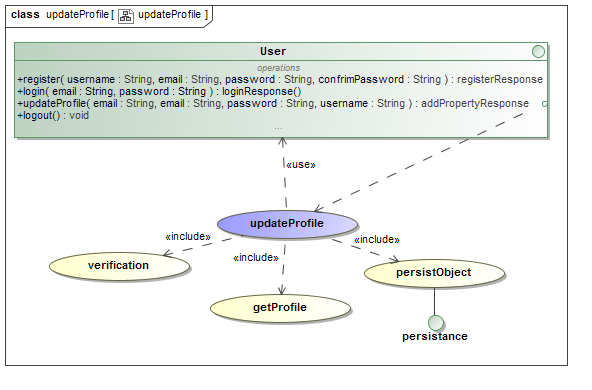
\includegraphics[width=1\textwidth]{./Images/newDiagrams/requiredFunctionality/Diana/updateProfile.png}
%Diana's Setion - End

% Kudzai's Section - starts
\subsubsection{addProperty}
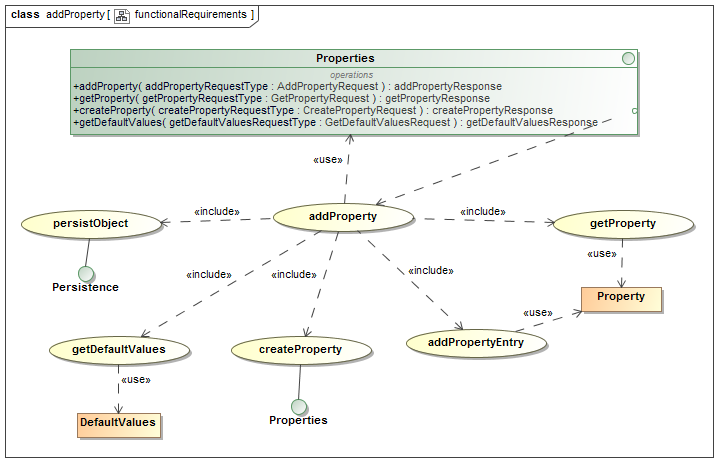
\includegraphics[width=1\textwidth]{./Images/requiredFunctionality/addProperty.png}
\subsubsection{deleteProperty}
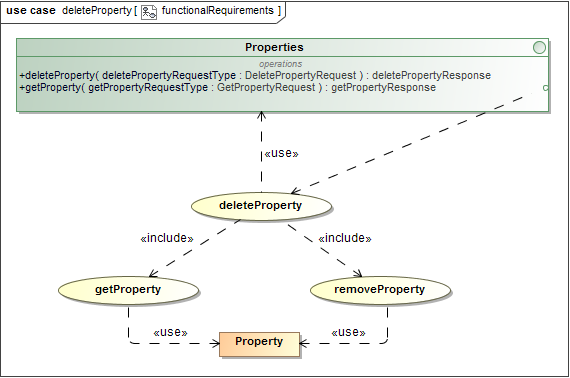
\includegraphics[width=1\textwidth]{./Images/requiredFunctionality/deleteProperty.png}
\subsubsection{updateProperty}
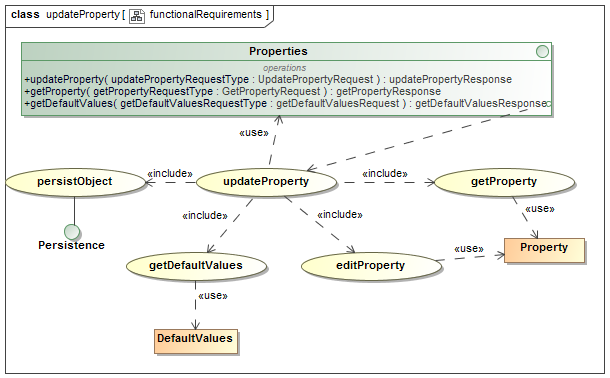
\includegraphics[width=1\textwidth]{./Images/requiredFunctionality/updateProperty.png}
\subsubsection{compareTwoProperties}
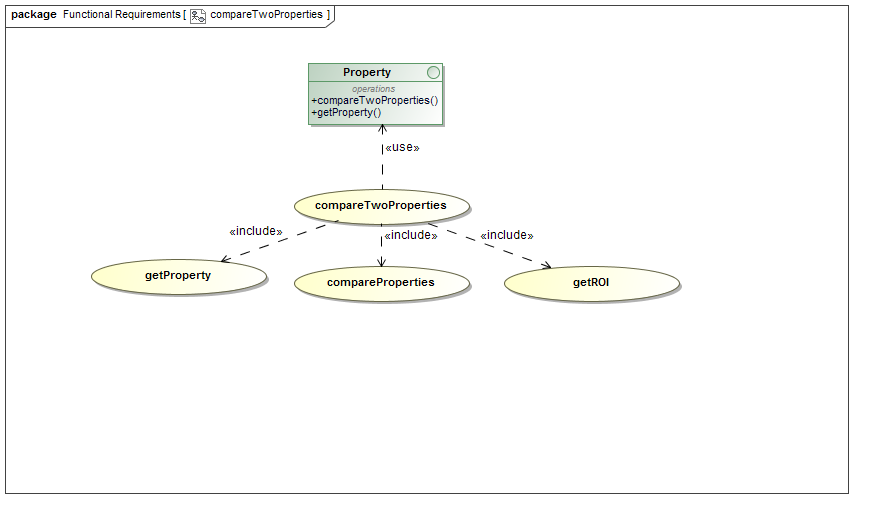
\includegraphics[width=1\textwidth]{./Images/requiredFunctionality/compareTwoProperties.png}
\subsubsection{viewProperty}
% Kudzai's Section - end

%Priscilla's Section (Required Functionality) - Start
\subsubsection{calucalateNPV}
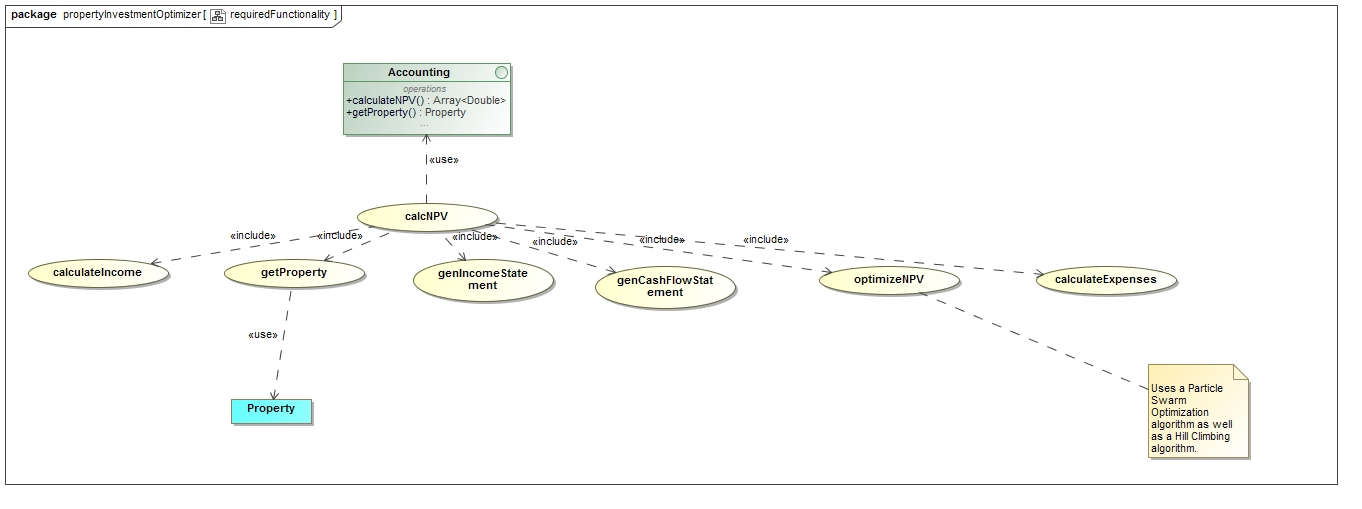
\includegraphics[width=1\textwidth]{./Images/newDiagrams/requiredFunctionality/Priscilla/requiredFunctionalityNPV.jpg}
\subsubsection{calucalateROI}
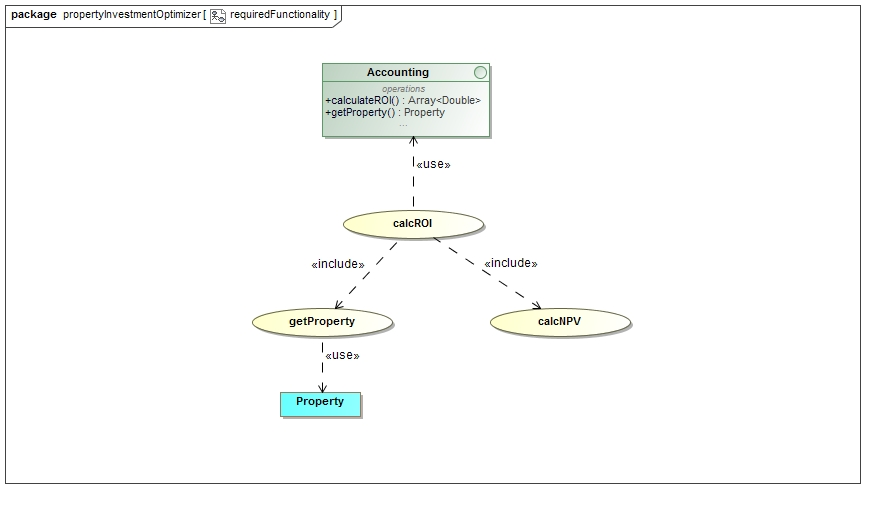
\includegraphics[width=1\textwidth]{./Images/newDiagrams/requiredFunctionality/Priscilla/requiredFunctionalityROI.jpg}
%Priscilla's Section (Required Functionality) - End

% Sandile's Section - starts
\subsubsection{generateReport}
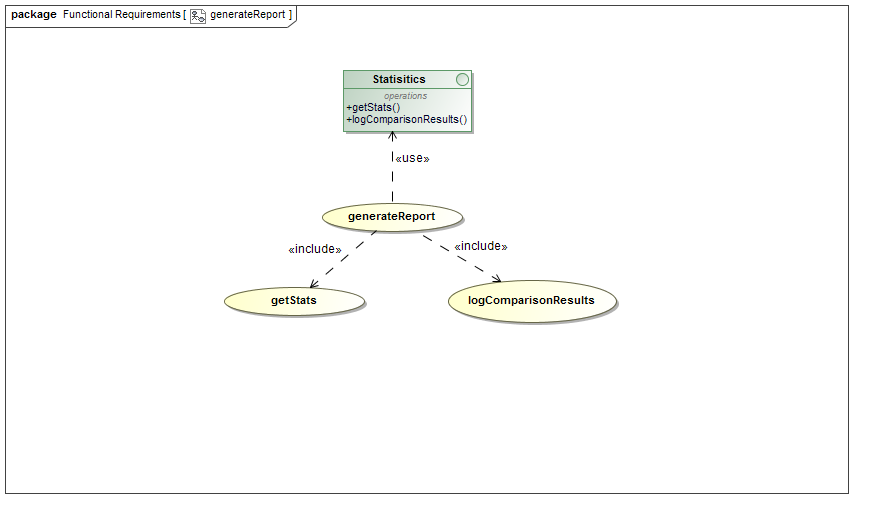
\includegraphics[width=1\textwidth]{./Images/requiredFunctionality/generateReport.png}
\subsubsection{viewReport}
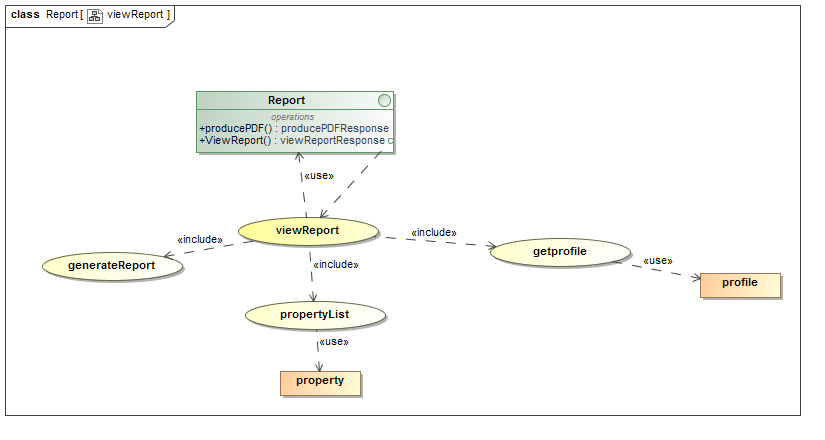
\includegraphics[width=1\textwidth]{./Images/newDiagrams/requiredFunctionality/Sandile/viewReportFR.png}
\subsubsection{generatePDF}
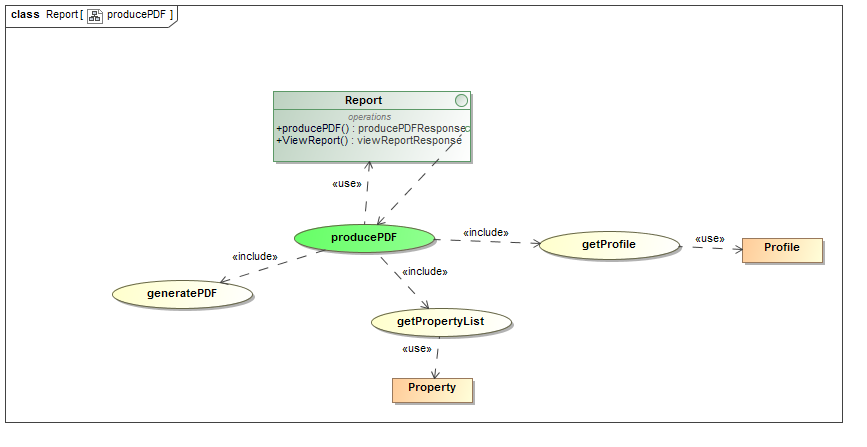
\includegraphics[width=1\textwidth]{./Images/newDiagrams/requiredFunctionality/Sandile/producePDFFR.png}

% Sandile's Section - end

\subsection{Process specifications}
%Diana's Section - Start
\subsubsection{Login}
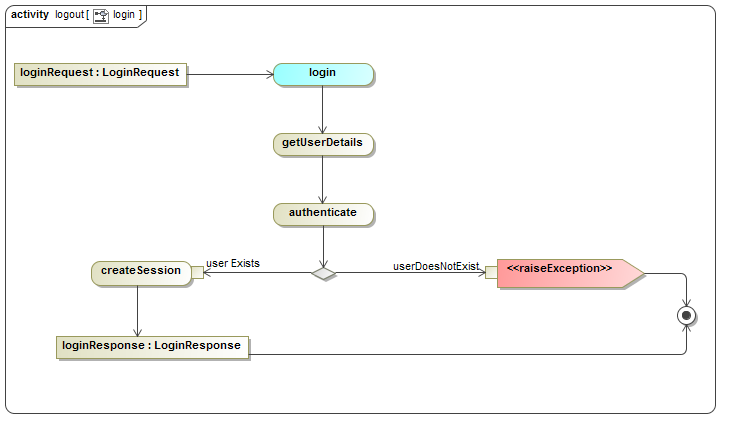
\includegraphics[width=1\textwidth]{./Images/newDiagrams/processSpecification/Diana/login.png}
\subsubsection{Logout}
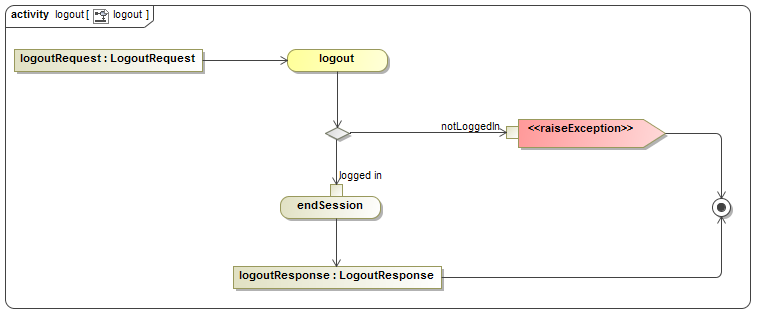
\includegraphics[width=1\textwidth]{./Images/newDiagrams/processSpecification/Diana/logout.png}
\subsubsection{Register}
\includegraphics[width=1\textwidth]{./Images/newDiagrams/processSpecification/Diana/register.png}
\subsubsection{updateProfile}
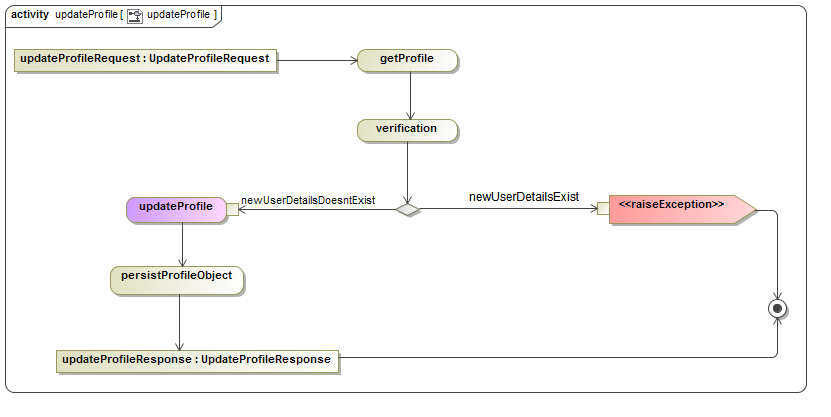
\includegraphics[width=1\textwidth]{./Images/newDiagrams/processSpecification/Diana/updateProfile.png}
%Diana's Section - End

% Kudzai's Section - starts
\subsubsection{addProperty}
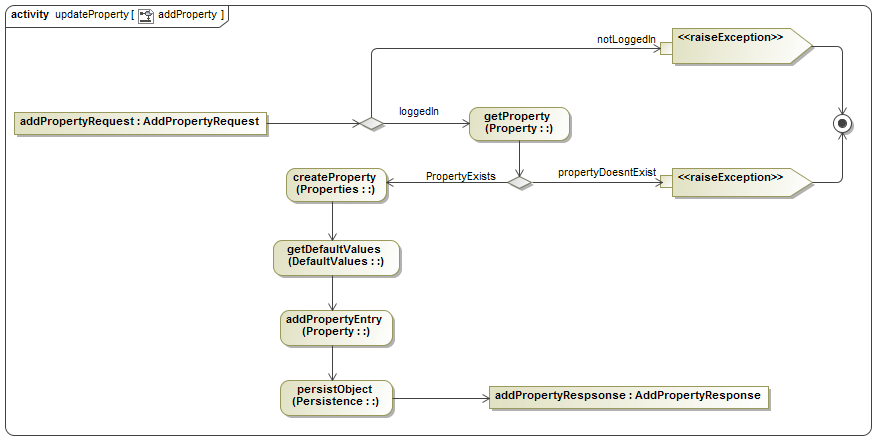
\includegraphics[width=1\textwidth]{./Images/processSpecification/addProperty.png}
\subsubsection{deleteProperty}
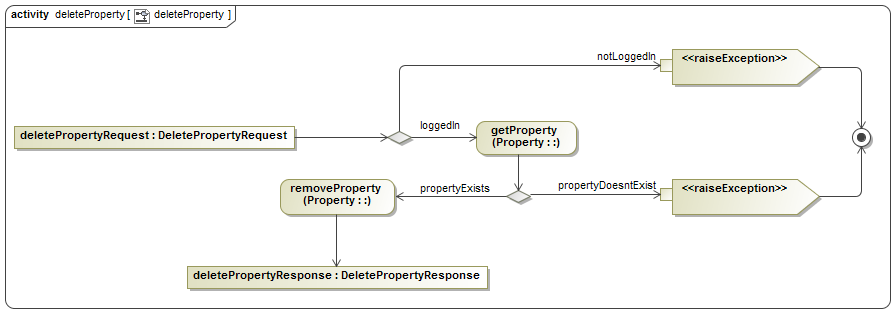
\includegraphics[width=1\textwidth]{./Images/processSpecification/deleteProperty.png}
\subsubsection{updateProperty}
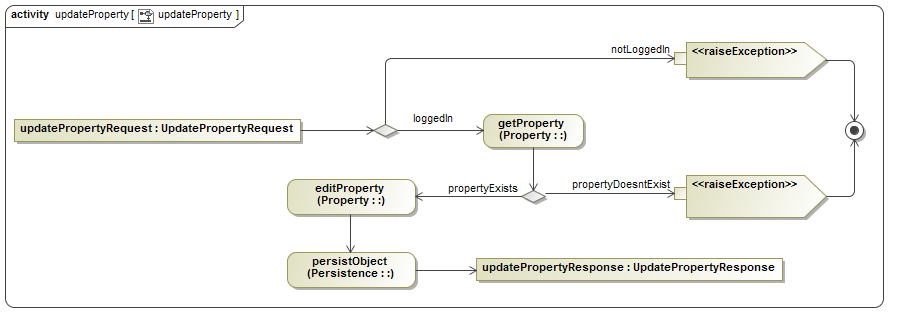
\includegraphics[width=1\textwidth]{./Images/processSpecification/updateProperty.png}
\subsubsection{compareTwoProperties}
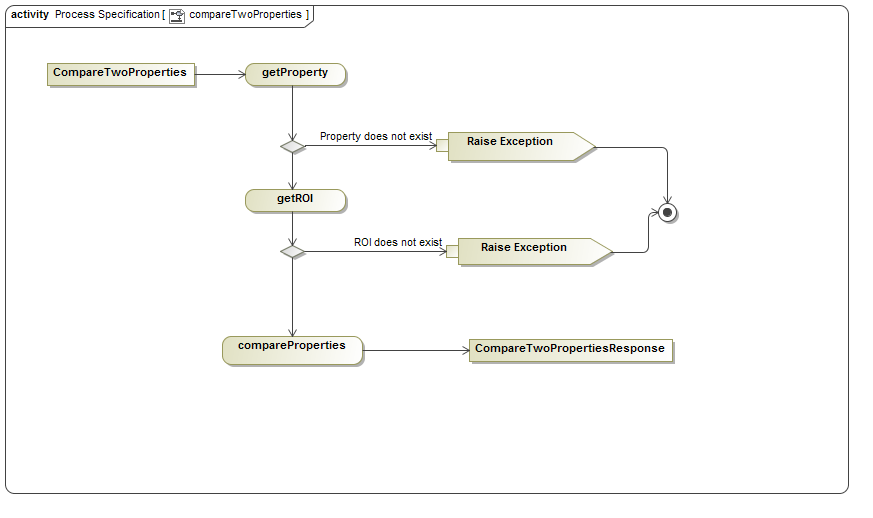
\includegraphics[width=1\textwidth]{./Images/processSpecification/compareTwoProperties.png}
\subsubsection{viewProperty}
% Kudzai's Section - end

%Priscilla's Section (Process Specification) - Start
\subsubsection{calucalateNPV}
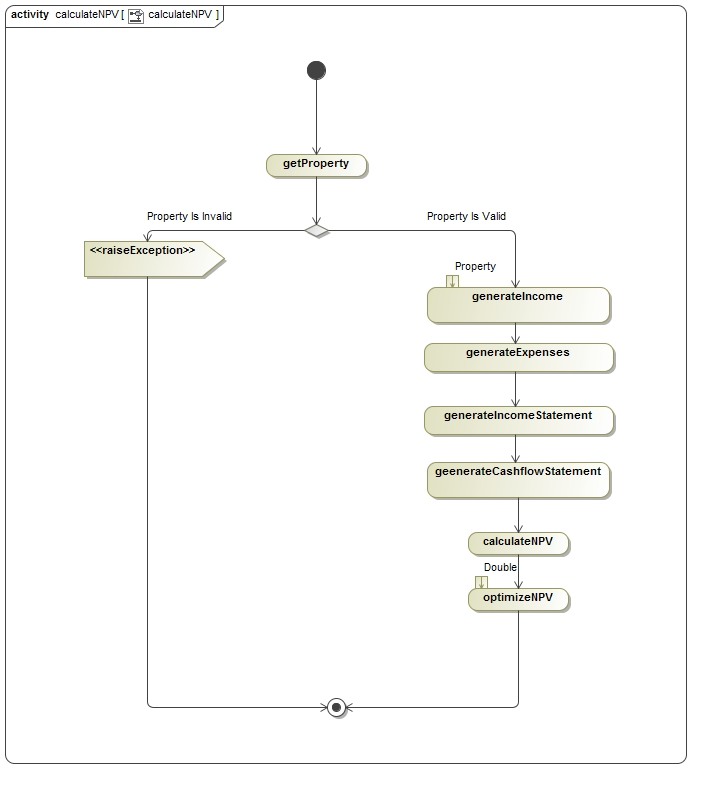
\includegraphics[width=1\textwidth]{./Images/newDiagrams/processSpecification/Priscilla/calculateNPV.jpg}
\subsubsection{calucalateROI}
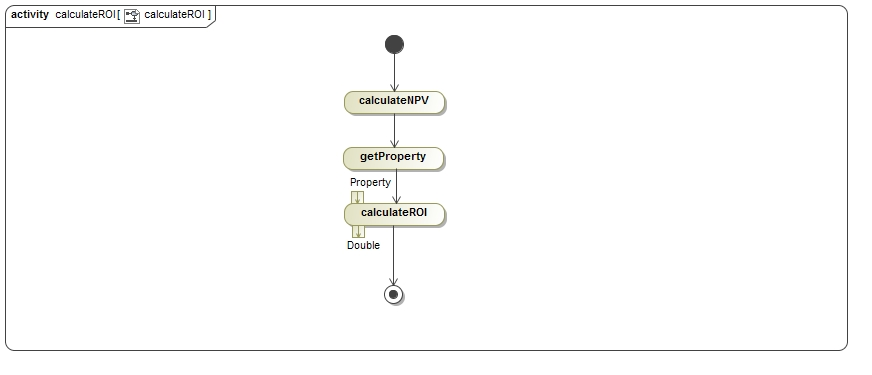
\includegraphics[width=1\textwidth]{./Images/newDiagrams/processSpecification/Priscilla/calculateROI.jpg}
%Priscilla's Section (Process Specification) - End

% Sandile's Section - starts
\subsubsection{generateReport}
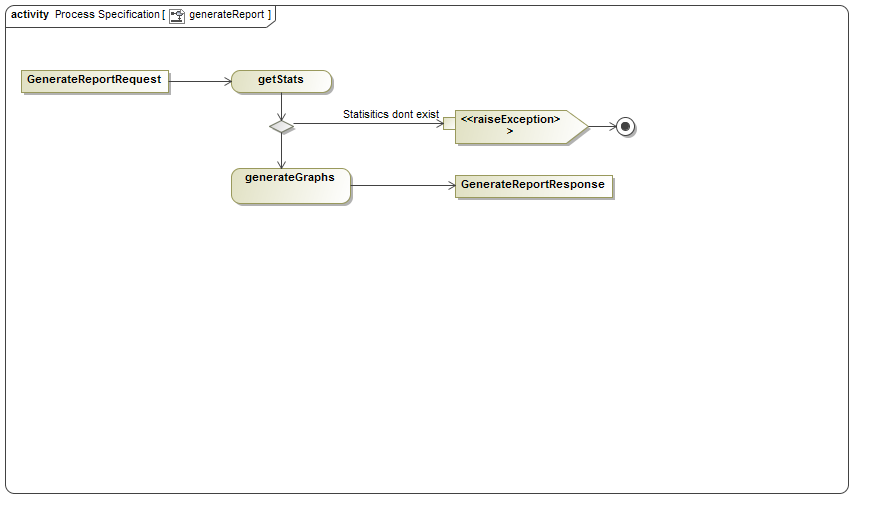
\includegraphics[width=1\textwidth]{./Images/processSpecification/generateReport.png}
\subsubsection{viewReport}
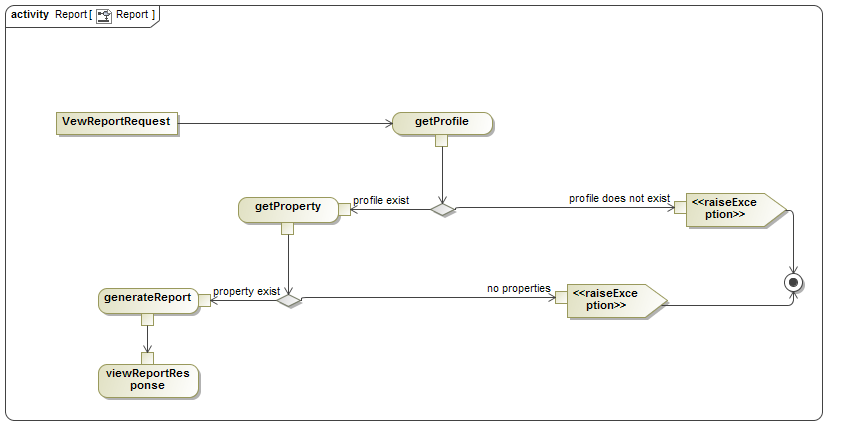
\includegraphics[width=1\textwidth]{./Images/newDiagrams/processSpecification/Sandile/viewReport.png}
\subsubsection{generatePDF}
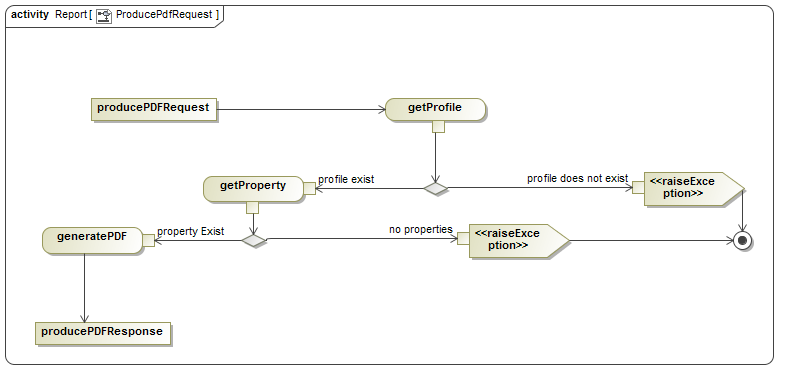
\includegraphics[width=1\textwidth]{./Images/newDiagrams/processSpecification/Sandile/ProducePdfRequest.png}
% Sandile's Section - end

\subsection{Domain Model}
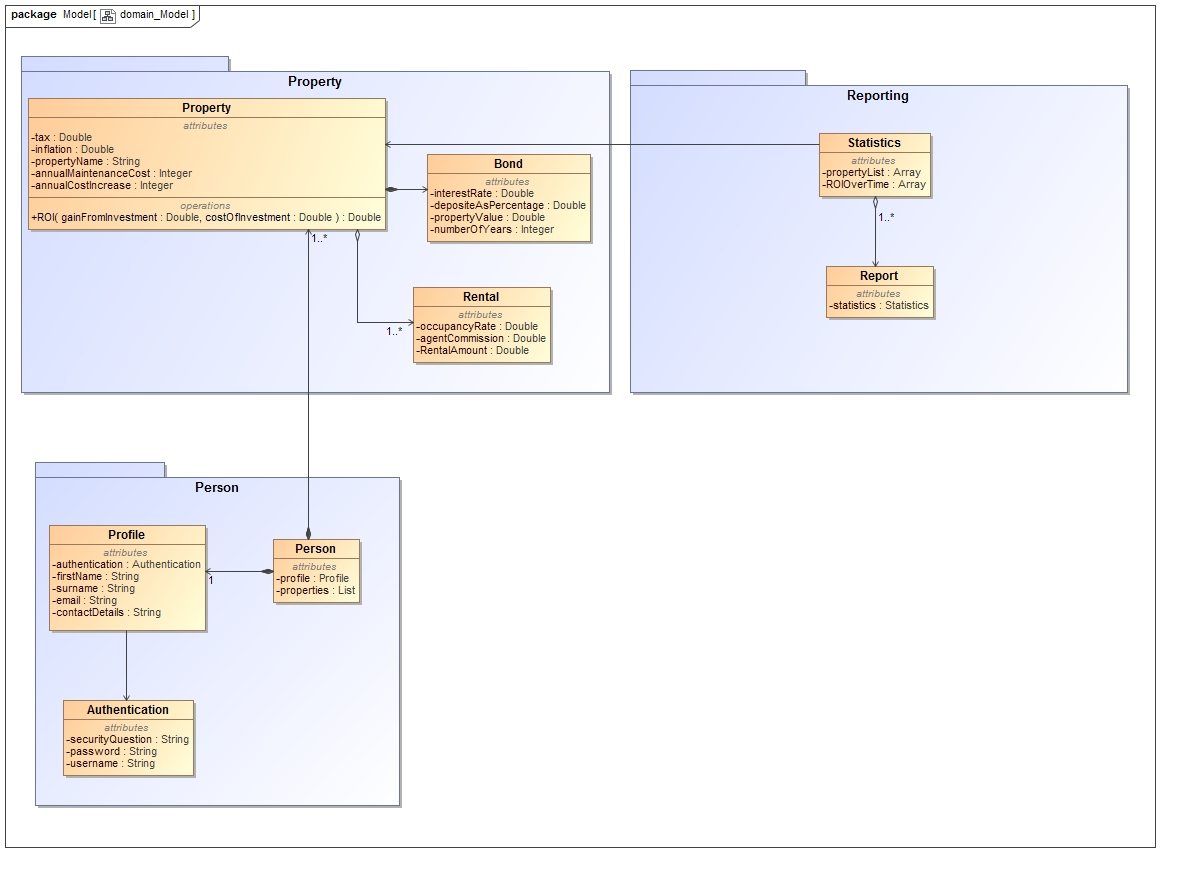
\includegraphics[width=1\textwidth]{./domainModel/domain_Model.PNG}


\newpage
\section{Open Issues}
\begin{itemize}
	\item An appropriate Particle Swarm Optimization algorithm API and a Hill Climbing API is needed to optimize the Net Present Value calculation. 
	\item We still need to get the EJB Container and JNDI lookup to work with our system.
\end{itemize}
\end{document}

